\documentclass{standalone}
\usepackage{tikz}
\usetikzlibrary{patterns, positioning}
\usepackage[sfdefault]{ClearSans} %% option 'sfdefault' activates Clear Sans as the default text font
\usepackage[T1]{fontenc}

\begin{document}
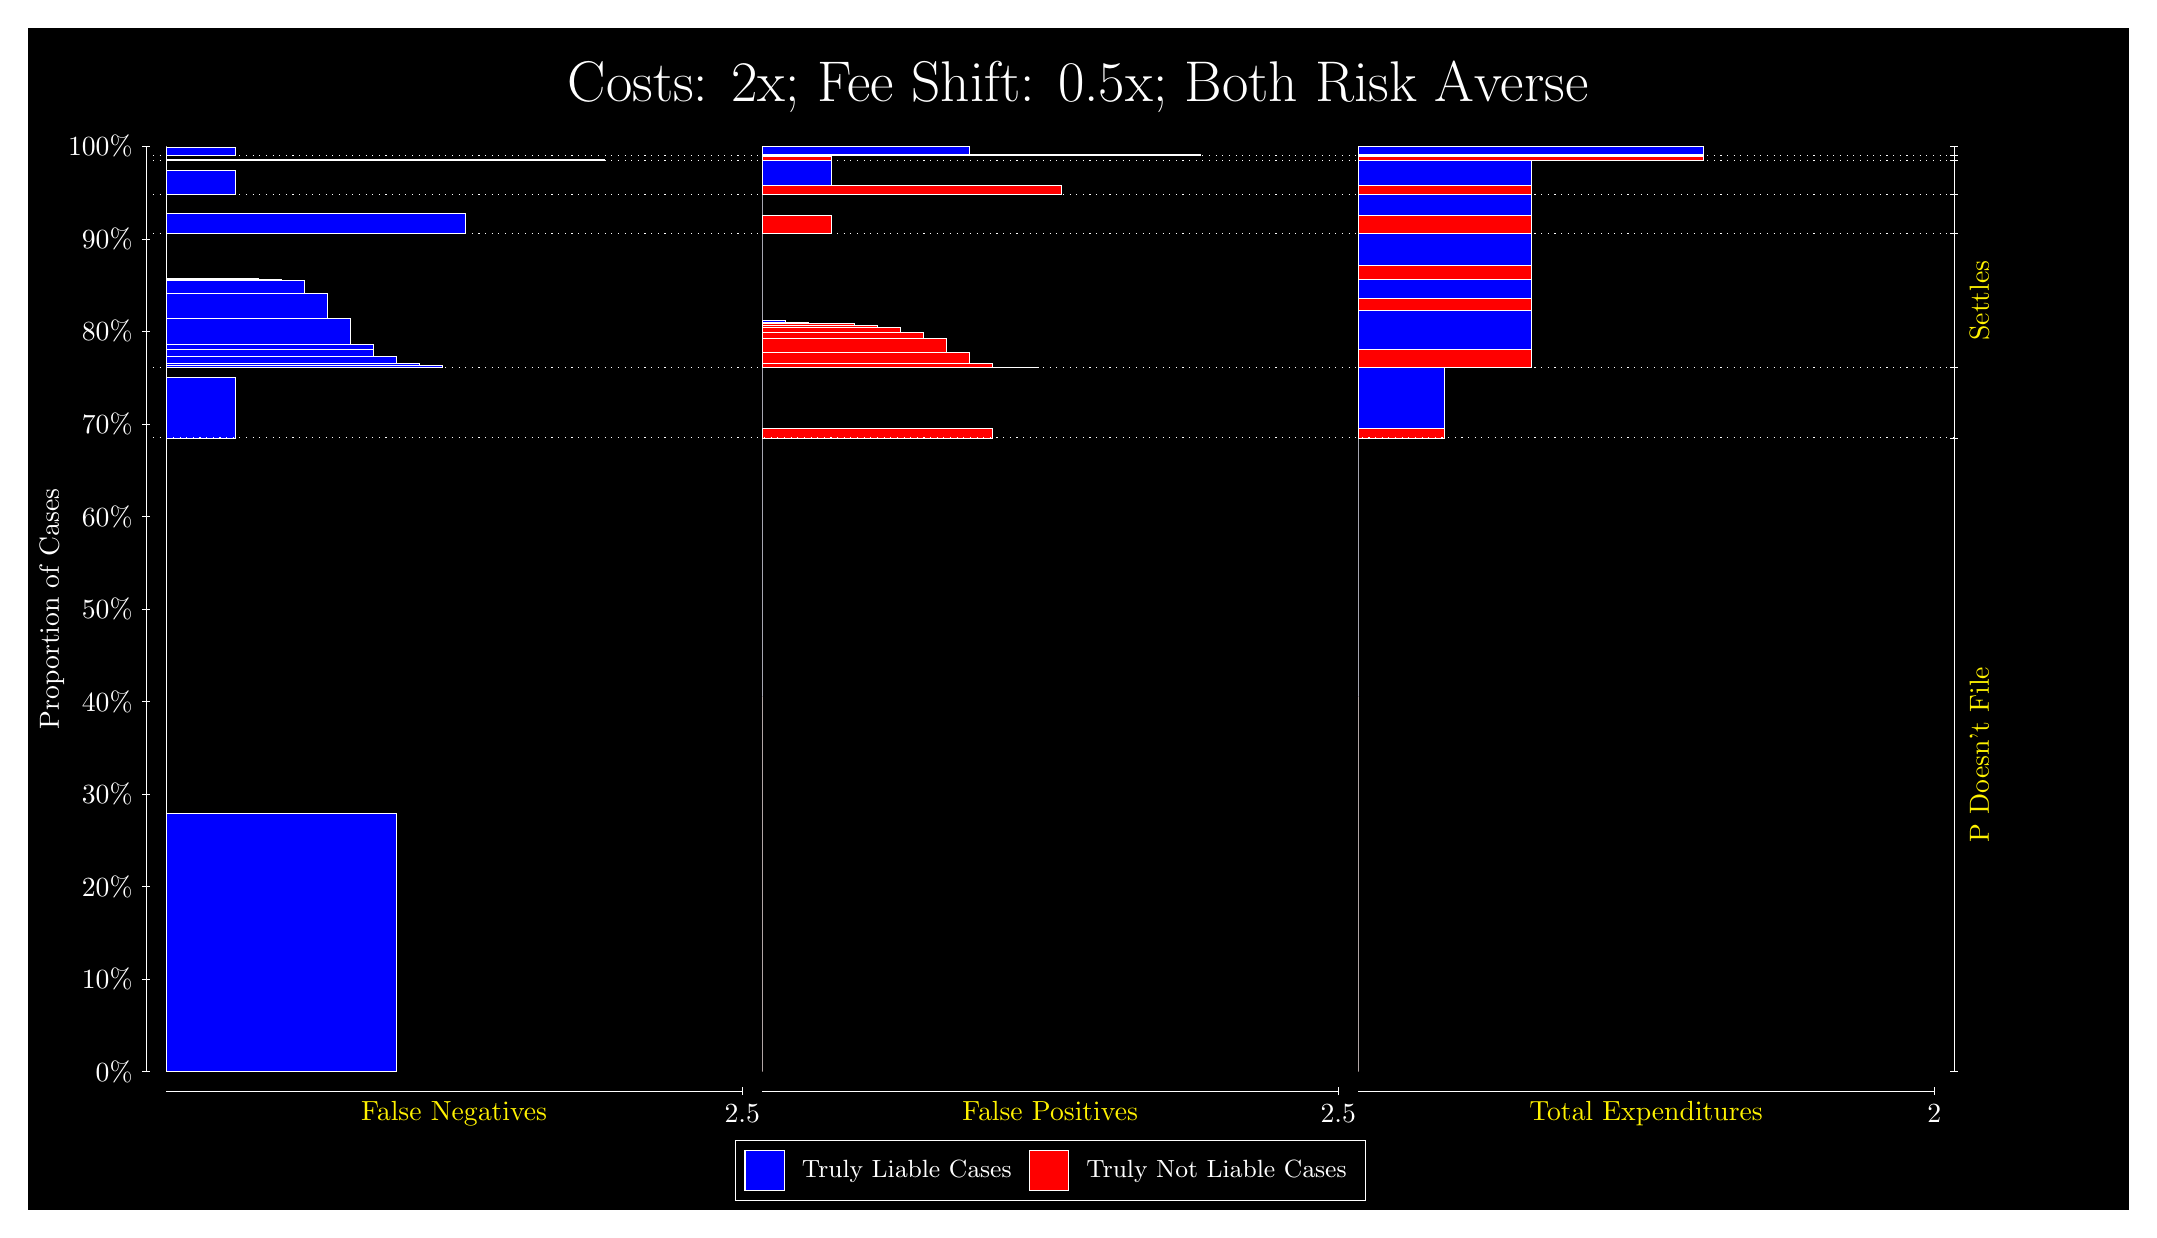
\begin{tikzpicture}
\draw[fill=black] (0,0) rectangle (26.667,15);
\draw[text=white] (0,13.5) rectangle (26.667,15) node[midway] {\huge Costs: 2x; Fee Shift: 0.5x; Both Risk Averse};
\draw[white, very thin] (1.5,1.75) -- (1.5,13.5);
\node[rotate=90, text=white, anchor=center] at (0.3, 7.625) {Proportion of Cases};
\draw[white, very thin] (1.45,1.75) -- (1.55,1.75);
\node[text=white, anchor=east] at (1.45, 1.75) {0\%};
\draw[white, very thin] (1.45,2.925) -- (1.55,2.925);
\node[text=white, anchor=east] at (1.45, 2.925) {10\%};
\draw[white, very thin] (1.45,4.1) -- (1.55,4.1);
\node[text=white, anchor=east] at (1.45, 4.1) {20\%};
\draw[white, very thin] (1.45,5.275) -- (1.55,5.275);
\node[text=white, anchor=east] at (1.45, 5.275) {30\%};
\draw[white, very thin] (1.45,6.45) -- (1.55,6.45);
\node[text=white, anchor=east] at (1.45, 6.45) {40\%};
\draw[white, very thin] (1.45,7.625) -- (1.55,7.625);
\node[text=white, anchor=east] at (1.45, 7.625) {50\%};
\draw[white, very thin] (1.45,8.8) -- (1.55,8.8);
\node[text=white, anchor=east] at (1.45, 8.8) {60\%};
\draw[white, very thin] (1.45,9.975) -- (1.55,9.975);
\node[text=white, anchor=east] at (1.45, 9.975) {70\%};
\draw[white, very thin] (1.45,11.15) -- (1.55,11.15);
\node[text=white, anchor=east] at (1.45, 11.15) {80\%};
\draw[white, very thin] (1.45,12.325) -- (1.55,12.325);
\node[text=white, anchor=east] at (1.45, 12.325) {90\%};
\draw[white, very thin] (1.45,13.5) -- (1.55,13.5);
\node[text=white, anchor=east] at (1.45, 13.5) {100\%};

\draw[white, very thin] (24.457,1.75) -- (24.457,13.5);
\draw[white, very thin] (24.407,1.75) -- (24.507,1.75);
\node[anchor=west] at (24.407, 1.75) {};
\draw[white, very thin] (24.407,9.7972) -- (24.507,9.7972);
\node[anchor=west] at (24.407, 9.7972) {};
\draw[white, very thin] (24.407,10.688) -- (24.507,10.688);
\node[anchor=west] at (24.407, 10.688) {};
\draw[white, very thin] (24.407,12.394) -- (24.507,12.394);
\node[anchor=west] at (24.407, 12.394) {};
\draw[white, very thin] (24.407,12.887) -- (24.507,12.887);
\node[anchor=west] at (24.407, 12.887) {};
\draw[white, very thin] (24.407,13.322) -- (24.507,13.322);
\node[anchor=west] at (24.407, 13.322) {};
\draw[white, very thin] (24.407,13.386) -- (24.507,13.386);
\node[anchor=west] at (24.407, 13.386) {};
\draw[white, very thin] (24.407,13.5) -- (24.507,13.5);
\node[anchor=west] at (24.407, 13.5) {};

\draw[white, very thin, fill=blue] (1.75,1.75) rectangle (4.6775,5.0338);
\draw[white, very thin, fill=red] (1.75,5.0338) rectangle (1.75,9.7972);
\draw[white, very thin, fill=blue] (1.75,9.7972) rectangle (2.6283,10.563);
\draw[white, very thin, fill=red] (1.75,10.563) rectangle (1.75,10.688);
\draw[white, very thin, fill=blue] (1.75,10.688) rectangle (5.2631,10.718);
\draw[white, very thin, fill=blue] (1.75,10.718) rectangle (4.9703,10.742);
\draw[white, very thin, fill=blue] (1.75,10.742) rectangle (4.6775,10.831);
\draw[white, very thin, fill=blue] (1.75,10.831) rectangle (4.3848,10.925);
\draw[white, very thin, fill=blue] (1.75,10.925) rectangle (4.3848,10.989);
\draw[white, very thin, fill=blue] (1.75,10.989) rectangle (4.092,11.311);
\draw[white, very thin, fill=blue] (1.75,11.311) rectangle (3.7993,11.634);
\draw[white, very thin, fill=blue] (1.75,11.634) rectangle (3.5065,11.795);
\draw[white, very thin, fill=blue] (1.75,11.795) rectangle (3.2138,11.81);
\draw[white, very thin, fill=blue] (1.75,11.81) rectangle (2.921,11.829);
\draw[white, very thin, fill=red] (1.75,11.829) rectangle (1.75,12.394);
\draw[white, very thin, fill=blue] (1.75,12.394) rectangle (5.5558,12.653);
\draw[white, very thin, fill=red] (1.75,12.653) rectangle (1.75,12.887);
\draw[white, very thin, fill=blue] (1.75,12.887) rectangle (2.6283,13.199);
\draw[white, very thin, fill=red] (1.75,13.199) rectangle (1.75,13.322);
\draw[white, very thin, fill=blue] (1.75,13.322) rectangle (7.3123,13.339);
\draw[white, very thin, fill=red] (1.75,13.339) rectangle (1.75,13.386);
\draw[white, very thin, fill=blue] (1.75,13.386) rectangle (2.6283,13.482);
\draw[white, very thin, fill=red] (1.75,13.482) rectangle (1.75,13.5);
\draw[white, very thin, fill=red] (9.3189,1.75) rectangle (9.3189,6.5134);
\draw[white, very thin, fill=blue] (9.3189,6.5134) rectangle (9.3189,9.7972);
\draw[white, very thin, fill=red] (9.3189,9.7972) rectangle (12.246,9.9219);
\draw[white, very thin, fill=blue] (9.3189,9.9219) rectangle (9.3189,10.688);
\draw[white, very thin, fill=red] (9.3189,10.688) rectangle (12.832,10.692);
\draw[white, very thin, fill=red] (9.3189,10.692) rectangle (12.539,10.696);
\draw[white, very thin, fill=red] (9.3189,10.696) rectangle (12.246,10.749);
\draw[white, very thin, fill=red] (9.3189,10.749) rectangle (11.954,10.884);
\draw[white, very thin, fill=red] (9.3189,10.884) rectangle (11.661,11.058);
\draw[white, very thin, fill=red] (9.3189,11.058) rectangle (11.368,11.134);
\draw[white, very thin, fill=red] (9.3189,11.134) rectangle (11.075,11.203);
\draw[white, very thin, fill=red] (9.3189,11.203) rectangle (10.783,11.233);
\draw[white, very thin, fill=red] (9.3189,11.233) rectangle (10.49,11.253);
\draw[white, very thin, fill=blue] (9.3189,11.253) rectangle (9.9044,11.271);
\draw[white, very thin, fill=blue] (9.3189,11.271) rectangle (9.6116,11.287);
\draw[white, very thin, fill=blue] (9.3189,11.287) rectangle (9.3189,12.394);
\draw[white, very thin, fill=red] (9.3189,12.394) rectangle (10.197,12.628);
\draw[white, very thin, fill=blue] (9.3189,12.628) rectangle (9.3189,12.887);
\draw[white, very thin, fill=red] (9.3189,12.887) rectangle (13.125,13.01);
\draw[white, very thin, fill=blue] (9.3189,13.01) rectangle (10.197,13.322);
\draw[white, very thin, fill=red] (9.3189,13.322) rectangle (10.197,13.368);
\draw[white, very thin, fill=blue] (9.3189,13.368) rectangle (9.3189,13.386);
\draw[white, very thin, fill=red] (9.3189,13.386) rectangle (14.881,13.403);
\draw[white, very thin, fill=blue] (9.3189,13.403) rectangle (11.954,13.5);
\draw[white, very thin, fill=red] (16.888,1.75) rectangle (16.888,6.5134);
\draw[white, very thin, fill=blue] (16.888,6.5134) rectangle (16.888,9.7972);
\draw[white, very thin, fill=red] (16.888,9.7972) rectangle (17.986,9.9219);
\draw[white, very thin, fill=blue] (16.888,9.9219) rectangle (17.986,10.688);
\draw[white, very thin, fill=red] (16.888,10.688) rectangle (19.083,10.919);
\draw[white, very thin, fill=blue] (16.888,10.919) rectangle (19.083,11.417);
\draw[white, very thin, fill=red] (16.888,11.417) rectangle (19.083,11.574);
\draw[white, very thin, fill=blue] (16.888,11.574) rectangle (19.083,11.811);
\draw[white, very thin, fill=red] (16.888,11.811) rectangle (19.083,11.988);
\draw[white, very thin, fill=blue] (16.888,11.988) rectangle (19.083,12.394);
\draw[white, very thin, fill=red] (16.888,12.394) rectangle (19.083,12.628);
\draw[white, very thin, fill=blue] (16.888,12.628) rectangle (19.083,12.887);
\draw[white, very thin, fill=red] (16.888,12.887) rectangle (19.083,13.01);
\draw[white, very thin, fill=blue] (16.888,13.01) rectangle (19.083,13.322);
\draw[white, very thin, fill=red] (16.888,13.322) rectangle (21.279,13.368);
\draw[white, very thin, fill=blue] (16.888,13.368) rectangle (21.279,13.386);
\draw[white, very thin, fill=red] (16.888,13.386) rectangle (21.279,13.403);
\draw[white, very thin, fill=blue] (16.888,13.403) rectangle (21.279,13.5);
\draw[white, dotted] (1.5,9.7972) -- (24.457,9.7972);
\draw[white, dotted] (1.5,10.688) -- (24.457,10.688);
\draw[white, dotted] (1.5,12.394) -- (24.457,12.394);
\draw[white, dotted] (1.5,12.887) -- (24.457,12.887);
\draw[white, dotted] (1.5,13.322) -- (24.457,13.322);
\draw[white, dotted] (1.5,13.386) -- (24.457,13.386);
\draw[white, very thin] (1.75,1.5) -- (9.0689,1.5);
\node[text=yellow, anchor=north] at (5.4094, 1.5) {False Negatives};
\draw[white, very thin] (9.0689,1.45) -- (9.0689,1.55);
\node[text=white, anchor=north] at (9.0689, 1.45) {2.5};

\draw[white, very thin] (9.3189,1.5) -- (16.638,1.5);
\node[text=yellow, anchor=north] at (12.978, 1.5) {False Positives};
\draw[white, very thin] (16.638,1.45) -- (16.638,1.55);
\node[text=white, anchor=north] at (16.638, 1.45) {2.5};

\draw[white, very thin] (16.888,1.5) -- (24.207,1.5);
\node[text=yellow, anchor=north] at (20.547, 1.5) {Total Expenditures};
\draw[white, very thin] (24.207,1.45) -- (24.207,1.55);
\node[text=white, anchor=north] at (24.207, 1.45) {2};

\node[text=yellow, centered, rotate=90] at (24.777, 5.7736) {P Doesn't File};

\node[text=yellow, centered, rotate=90] at (24.777, 11.541) {Settles};





\draw (12.978300999999998,1.5) node[draw=none] (baseCoordinate) {};
\begin{scope}[align=center]
        \matrix[scale=0.5, draw=white, below=0.5cm of baseCoordinate, nodes={draw}, column sep=0.1cm]{
            \node[rectangle, draw, minimum width=0.5cm, minimum height=0.5cm, fill=blue] {}; &
            \node[draw=none, font=\small, text=white] (B) {Truly Liable Cases}; &
            \node[rectangle, draw, minimum width=0.5cm, minimum height=0.5cm, fill=red] {}; &
            \node[draw=none, font=\small, text=white] (B) {Truly Not Liable Cases}; \\
            };
\end{scope}

\end{tikzpicture}
\end{document}